
%(BEGIN_QUESTION)
% Copyright 2009, Tony R. Kuphaldt, released under the Creative Commons Attribution License (v 1.0)
% This means you may do almost anything with this work of mine, so long as you give me proper credit

In this process, maple syrup is heated as it passes through a steam heat exchanger, then enters an evaporator where the water boils off.  The purpose of this is to raise the sugar concentration of the syrup, making it suitable for use as a food topping.  A level control system (LT, LIC, and LV) maintains constant syrup level inside the evaporator, while an analytical control system (AT, AIR, AC, and AV) monitors the sugar concentration of the syrup and adjusts steam flow to the heat exchanger accordingly.

$$\includegraphics[width=15.5cm]{i04314x01.eps}$$

Suppose the analytical control loop has been optimally tuned, with the sugar concentration of the evaporated syrup holding precisely at setpoint.  Now suppose the steam supplied to this process by the boiler suddenly increases in temperature.  Explain what will happen to the syrup's sugar concentration over time, assuming two different control algorithms, all other factors being equal:

\vskip 10pt

\noindent
{\bf Analytical controller is proportional-only:}

\vskip 50pt

\noindent
{\bf Analytical controller is proportional-plus-integral (P+I):}

\vfil 

\underbar{file i04314}
\eject
%(END_QUESTION)





%(BEGIN_ANSWER)

This is a graded question -- no answers or hints given!

%(END_ANSWER)





%(BEGIN_NOTES)

A sudden increase in steam temperature constitutes a load to the sugar concentration loop.  A rise in temperature will drive more water from the syrup, increasing its sugar concentration.  The analyzer will sense this change, with the controller pinching down on the steam valve to compensate.  

\vskip 10pt

\noindent
{\bf Analytical controller is proportional-only:}

An offset will develop between PV and SP: sugar concentration will settle at a value slightly greater than setpoint.  This is because a proportional-only controller is incapable of automatically generating new (different) output values when PV=SP.  If a load drives PV off of setpoint, a new valve position will be required to check that deviation.  However, the only way a P-only controller can possibly generate a new output value is to let the PV deviate slightly from SP, and so an offset develops.

\vskip 10pt

\noindent
{\bf Analytical controller is proportional-plus-integral (P+I):}

Sugar concentration will initially rise above setpoint, then return exactly to setpoint, because integral action keeps driving the output to new values (as far as necessary) until all error between PV and SP is eliminated.


%INDEX% Basics, control loop troubleshooting: determining effect of process valve problem
%INDEX% Process: maple syrup concentration (single-effect evaporator)

%(END_NOTES)


